\documentclass[aspectratio=169,10pt]{beamer}

\usetheme{Madrid}
\setbeamertemplate{navigation symbols}{}
\setbeamertemplate{footline}[frame number]
\usepackage{hyperref}
\usepackage{amsmath}
\usepackage{amssymb}
\usepackage{array}
\usepackage{booktabs}
\usepackage{graphicx}
\usepackage{tabularx}
\usepackage{tikz}
\usetikzlibrary{arrows.meta,calc,positioning}

\graphicspath{{../data/}{../figures/}}

\definecolor{LectureBlue}{RGB}{13,76,100}
\definecolor{LectureTeal}{RGB}{0,118,122}
\definecolor{LectureGold}{RGB}{194,142,37}
\definecolor{Slate}{RGB}{58,68,84}
\definecolor{SoftGray}{RGB}{245,247,249}

\setbeamercolor{title}{fg=LectureBlue}
\setbeamercolor{subtitle}{fg=Slate}
\setbeamercolor{frametitle}{fg=LectureBlue,bg=LectureBlue!8}
\setbeamercolor{structure}{fg=LectureBlue}
\setbeamercolor{block title}{fg=white,bg=LectureBlue}
\setbeamercolor{block body}{fg=black,bg=SoftGray}
\setbeamercolor{alerted text}{fg=LectureGold}

\renewcommand{\arraystretch}{1.12}

\title{Digital Image Representation, Geometry, and Resampling}
\author{}
\date{May 2026}

\begin{document}

\begin{frame}[plain]
\begin{columns}[c,onlytextwidth]
\column{0.58\textwidth}
{\usebeamerfont{title}\color{LectureBlue}\inserttitle\par}
\vspace{0.4em}
{\usebeamerfont{subtitle}\color{Slate}\insertsubtitle\par}

{\small \insertauthor \hfill \insertdate}

\column{0.38\textwidth}
\includegraphics[width=\linewidth]{ct.jpeg}
\end{columns}
\end{frame}

\begin{frame}{Contents}

\begin{itemize}
\item Digital image formation as a sequence of operators
\item Sampling, quantization, and geometric resampling as information-processing steps
\item Coordinate systems, transform models, and interpolation
\item Why these classical choices still matter in deep learning
\end{itemize}



\end{frame}

\section{Sampling and Quantization}
\begin{frame}
\centering
\vspace{0.25\textheight}
{\Huge Sampling, Quantization, and Resampling}
\end{frame}

\begin{frame}
\begin{center}
  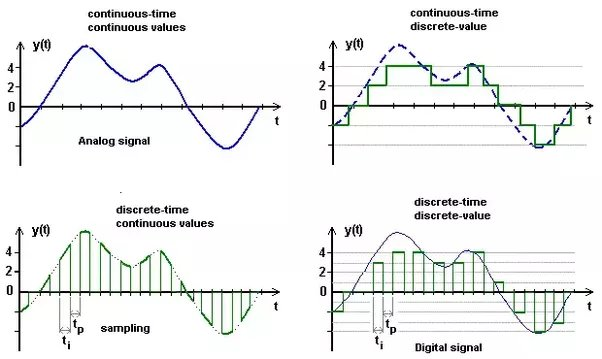
\includegraphics[height=1\textheight]{../figures/sampling_quantile.png}

\end{center}

\end{frame}




\begin{frame}{Image processing as a Operator}
\begin{columns}[T,onlytextwidth]
\column{0.58\textwidth}
\[
\mathbf{y} = Q\Bigl(S\bigl(h * g\bigr) \Bigr)
\]
\vspace{-0.5em}
\begin{itemize}
\item $g$: underlying continuous scene or object
\item $h$: imaging blur or point-spread function or some filtering operation
\item $S$: spatial sampling operator
\item $Q$: quantization to a discrete numeric representation
\end{itemize}


\column{0.37\textwidth}
\centering
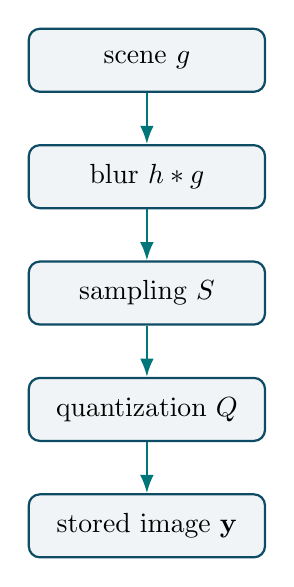
\begin{tikzpicture}[node distance=0.65cm,>=Latex]
\tikzstyle{stage}=[draw=LectureBlue,rounded corners,thick,minimum width=3.0cm,minimum height=0.8cm,fill=LectureBlue!6]
\node[stage] (scene) {scene $g$};
\node[stage,below=of scene] (blur) {blur $h*g$};
\node[stage,below=of blur] (sample) {sampling $S$};
\node[stage,below=of sample] (quantize) {quantization $Q$};
\node[stage,below=of quantize] (image) {stored image $\mathbf{y}$};
\draw[->,thick,LectureTeal] (scene) -- (blur);
\draw[->,thick,LectureTeal] (blur) -- (sample);
\draw[->,thick,LectureTeal] (sample) -- (quantize);
\draw[->,thick,LectureTeal] (quantize) -- (image);
\end{tikzpicture}
\end{columns}
\end{frame}



\begin{frame}{Sampling as an Operator}
\begin{columns}[T,onlytextwidth]
\column{0.56\textwidth}
\[
g_s(x,y) = g(x,y) \sum_{m,n \in \mathbb{Z}} \delta(x-m\Delta_x)\delta(y-n\Delta_y)
\]
\vspace{-0.5em}
\begin{itemize}
\item Sampling is multiplication by a spatial impulse train.
\item In the frequency domain, this produces replicated spectra.
\item If replicas overlap, aliasing occurs and the overlap cannot be undone from the sampled image alone.
\end{itemize}

\begin{block}{Animation}
https://phiresky.github.io/convolution-demo/
\end{block}

\column{0.40\textwidth}
\centering
\begin{center}
  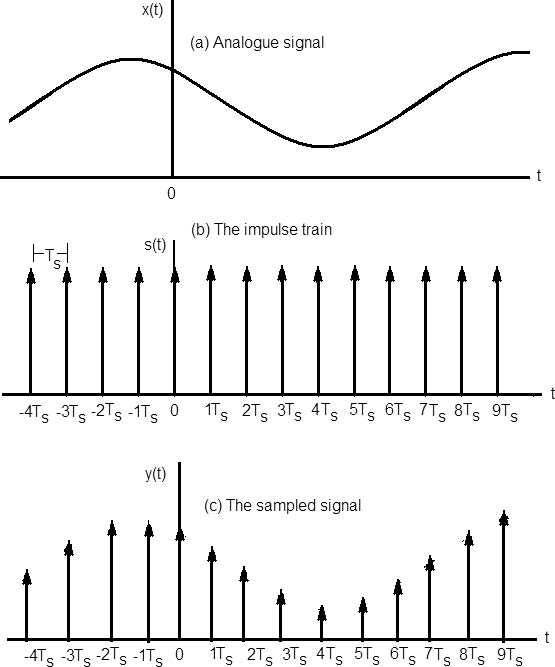
\includegraphics[width=0.8\linewidth]{../figures/sampling.png}

\end{center}
\end{columns}
\end{frame}

\begin{frame}
\begin{center}
  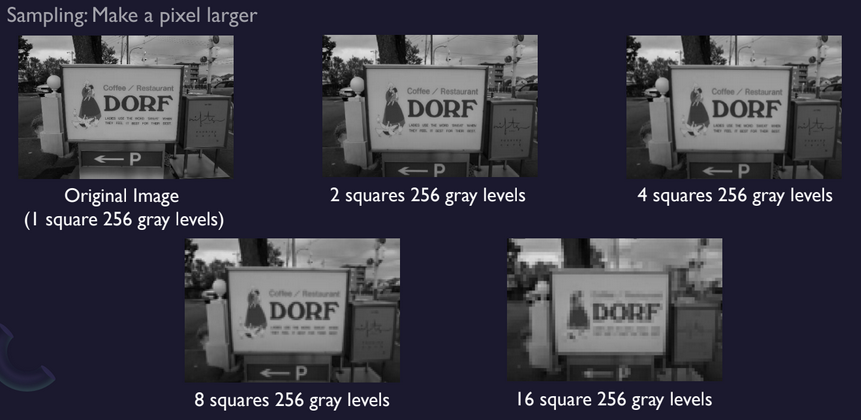
\includegraphics[width=1\linewidth]{../figures/sampling_viz.png}

\end{center}

\end{frame}

\begin{frame}{Nyquist, Aliasing, and the Cost of Undersampling}
\begin{columns}[T,onlytextwidth]
\column{0.55\textwidth}
\begin{itemize}
\item Smaller pixel spacing permits higher recoverable spatial frequency.
\item Equivalently, in frequency terms: $f_{s,x} = 1/\Delta_x \geq 2B_x$ and $f_{s,y} = 1/\Delta_y \geq 2B_y$ for scene frequency $B_x, B_y$.
\item Downsampling without prefiltering folds high frequencies into lower frequencies.
\item In scientific imaging, aliasing corrupts measurement, not just aesthetics.
\end{itemize}
\vspace{0.5em}
\begin{block}{}
Sample at least twice as fast as the highest spatial frequency you want to preserve, or suppress that frequency before sampling.
\end{block}

\column{0.40\textwidth}
\centering
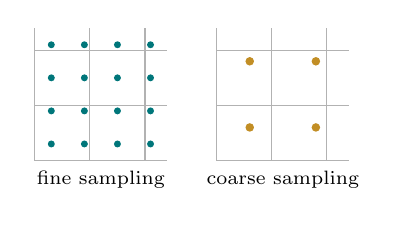
\begin{tikzpicture}[scale=0.7]
\draw[gray!60] (0,0) grid (2.4,2.4);
\foreach \x in {0.3,0.9,1.5,2.1}
  \foreach \y in {0.3,0.9,1.5,2.1}
    \fill[LectureTeal] (\x,\y) circle (1.8pt);
\node[font=\scriptsize] at (1.2,-0.35) {fine sampling};

\begin{scope}[xshift=3.3cm]
\draw[gray!60] (0,0) grid (2.4,2.4);
\foreach \x in {0.6,1.8}
  \foreach \y in {0.6,1.8}
    \fill[LectureGold] (\x,\y) circle (2.2pt);
\node[font=\scriptsize] at (1.2,-0.35) {coarse sampling};
\end{scope}
\end{tikzpicture}
\vspace{0.2em}

\includegraphics[height=0.23\textheight]{ct.jpeg}
\end{columns}
\end{frame}


\begin{frame}{Quantization Sets Intensity Resolution}

\begin{itemize}
\item Quantization maps a continuous intensity range to a finite set of gray levels.
\item An 8-bit image stores $2^8 = 256$ levels; a 12-bit image stores 4096 levels.
\item Too few levels create banding, contouring, or loss of subtle contrast.
\item Acquisition depth and display depth are not always the same: CT often stores more precision than we display at once.
\end{itemize}


\end{frame}


\begin{frame}
\begin{center}
  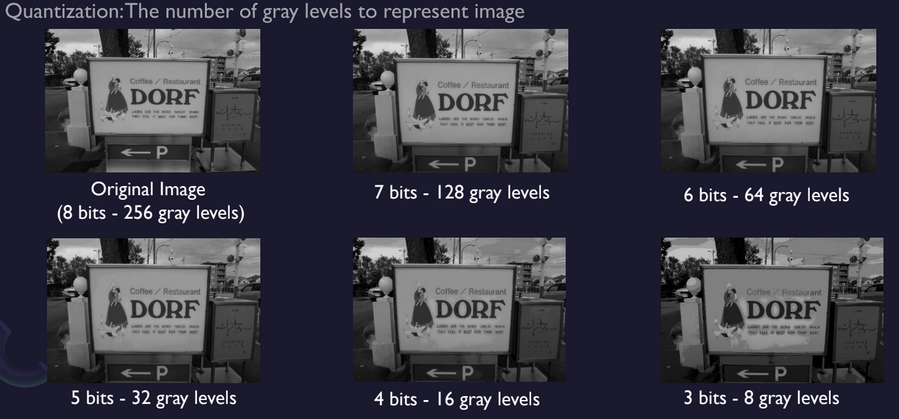
\includegraphics[width=1\linewidth]{../figures/quantile_viz.png}

\end{center}

\end{frame}

\begin{frame}{Information Loss and Invertibility}
\small
\begin{tabularx}{\textwidth}{>{\bfseries}p{0.2\textwidth} >{\raggedright\arraybackslash}p{0.22\textwidth} X}
\toprule
Operation & Invertible? & Reason \\
\midrule
Translation on an infinite grid & Often yes & It rearranges coordinates without collapsing distinct values. \\
Rotation plus interpolation & Approximate only & Interpolation introduces model-based approximation and boundary loss. \\
Downsampling & No & Multiple high-resolution images map to the same coarse image. \\
Quantization & No & Continuous intensity intervals collapse to the same stored value. \\
Cropping & No & Discarded spatial support is unavailable later. \\
\bottomrule
\end{tabularx}


\end{frame}

\begin{frame}{Common Artifacts From Poor Discretization}
\small
\begin{tabularx}{\textwidth}{>{\bfseries}p{0.23\textwidth} X}
\toprule
Artifact & Interpretation \\
\midrule
Aliasing & Sampling is too coarse for the spatial detail in the scene. Fine texture can appear as false low-frequency patterns. \\
Banding & Quantization is too coarse, so smooth intensity transitions become step-like. \\
\bottomrule
\end{tabularx}

\end{frame}

\begin{frame}
\begin{center}
  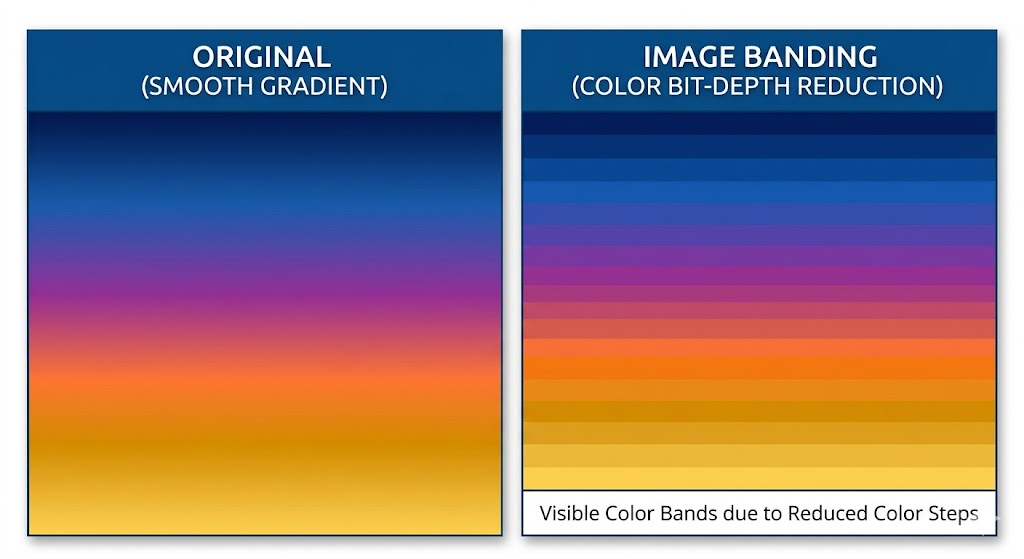
\includegraphics[width=1\linewidth]{../figures/image_banding.png}

\end{center}
\end{frame}

\begin{frame}
\begin{center}
  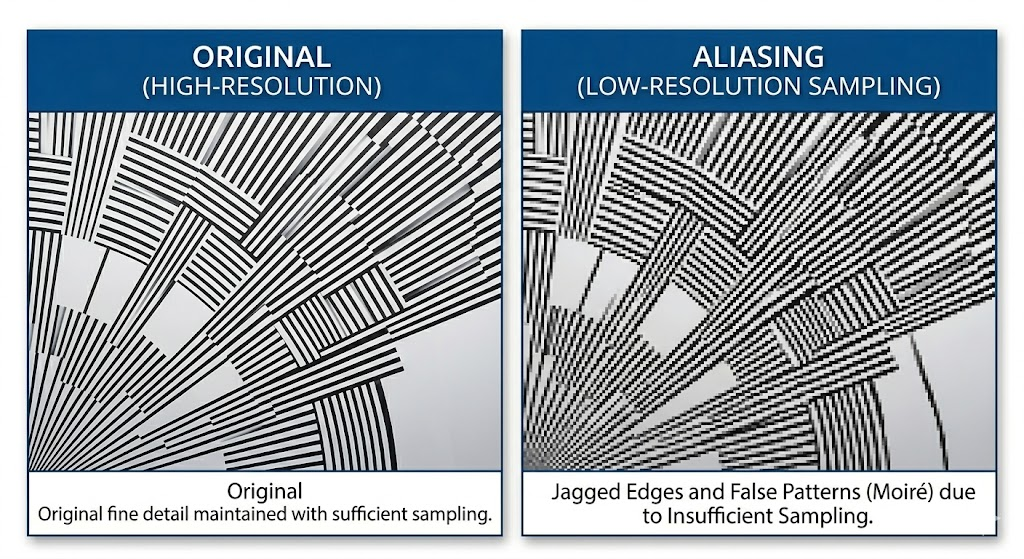
\includegraphics[width=1\linewidth]{../figures/image_aliasing.png}

\end{center}
\end{frame}

\section{Geometric operations}
\begin{frame}
\centering
\vspace{0.25\textheight}
{\Huge Geometric operations}
\end{frame}

\begin{frame}{Coordinate Systems}
\begin{columns}[T,onlytextwidth]
\column{0.50\textwidth}
\begin{itemize}
\item \textbf{Index space}: array coordinates such as $(i,j,k)$.
\item \textbf{Physical space}: coordinates measured in mm or another physical unit.
\end{itemize}


\column{0.44\textwidth}
\[
\mathbf{x}_{\mathrm{phys}} = D\,\mathbf{x}_{\mathrm{idx}} + \mathbf{o}
\]
\vspace{-0.5em}
\begin{itemize}
\item $D$: spacing and orientation
\item $\mathbf{o}$: origin
\end{itemize}
\end{columns}
\end{frame}

\begin{frame}{Geometric Transformations}
Geometric operations consist of two steps:
\begin{itemize}
  \item Spatial transformation of coordinates
  \item Intensity interpolation
\end{itemize}

\vspace{0.5cm}

\begin{itemize}
  \item \href{https://opencv24-python-tutorials.readthedocs.io/en/latest/py_tutorials/py_imgproc/py_geometric_transformations/py_geometric_transformations.html}{Transformation in OpenCV}
  \item \href{https://docs.opencv.org/3.4/da/d54/group__imgproc__transform.html\#ga5bb5a1fea74ea38e1a5445ca803ff121}{Interpolation in OpenCV}
\end{itemize}
\end{frame}

\begin{frame}{General Geometric Transformation}
\small
\[
T:\mathbb{R}^n \to \mathbb{R}^n,\qquad \mathbf{x}' = T(\mathbf{x}).
\]

Example forms:
\[
\text{Affine: } T(\mathbf{x}) = A\mathbf{x}+\mathbf{t},\quad A\in\mathbb{R}^{n\times n},\ \mathbf{t}\in\mathbb{R}^n.
\]
\[
\text{Projective (homogeneous): } \tilde{\mathbf{x}}' = H\tilde{\mathbf{x}},\quad H\in\mathbb{R}^{(n+1)\times(n+1)}.
\]

If $T$ is differentiable, its Jacobian $J_T(\mathbf{x})=\partial T/\partial\mathbf{x}$ gives the local linearization; $\det J_T$ scales volumes.

Composition and inverse:
\[
(T_2\circ T_1)(\mathbf{x}) = T_2(T_1(\mathbf{x})),\qquad T^{-1}\ \text{exists if }T\ \text{is bijective}.
\]

\end{frame}


\begin{frame}
\begin{center}
  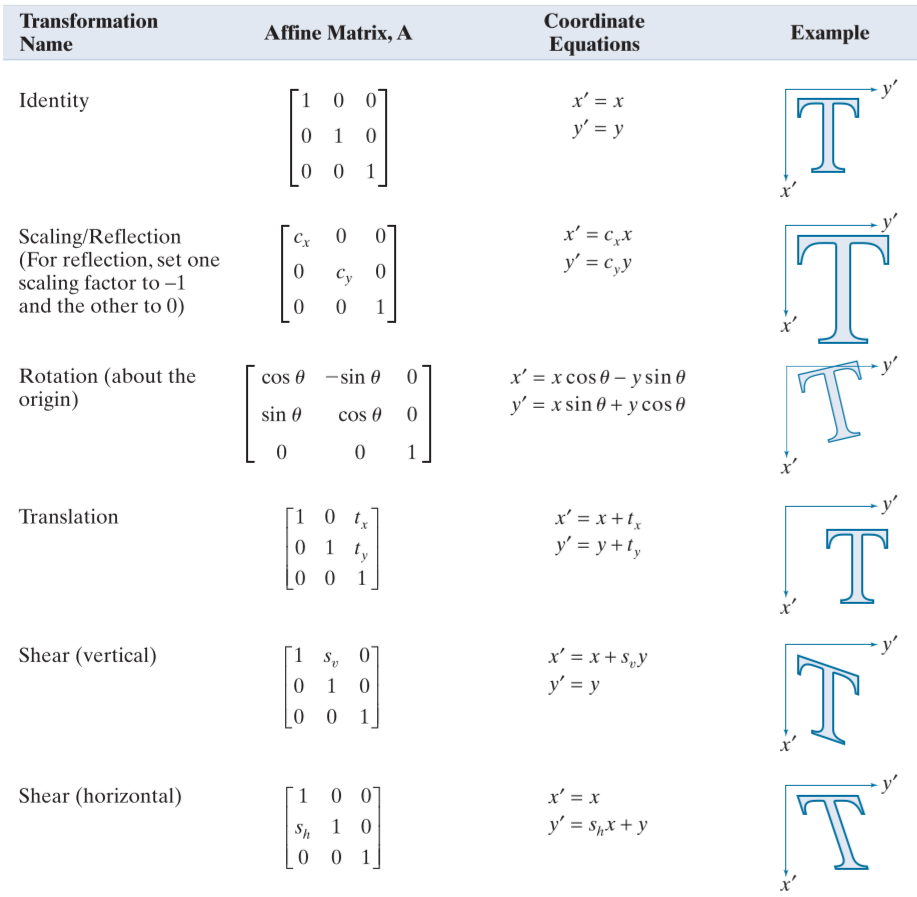
\includegraphics[width=0.6\linewidth]{../figures/trans.png}

\end{center}

\end{frame}


\begin{frame}{Geometric Transforms: What Changes and What Stays}
\small
\begin{tabularx}{\textwidth}{>{\bfseries}p{0.15\textwidth} >{\raggedright\arraybackslash}p{0.24\textwidth} >{\raggedright\arraybackslash}p{0.22\textwidth} X}
\toprule
Family & Form & Preserves & Typical use \\
\midrule
Rigid & $\mathbf{x}' = R\mathbf{x} + \mathbf{t}$ & distance and angle & translation and rotation \\
Similarity & $\mathbf{x}' = sR\mathbf{x} + \mathbf{t}$ & angle and overall shape & zoom plus rigid motion \\
Affine & $\mathbf{x}' = A\mathbf{x} + \mathbf{t}$ & straight lines and parallelism & scale, shear, skew \\
Projective & $\tilde{\mathbf{x}}' = H\tilde{\mathbf{x}}$ & straight lines & perspective correction, camera-plane mapping \\
\bottomrule
\end{tabularx}


\end{frame}

\begin{frame}{Affine Transformation (definition) -- Example}
\small
\[
\mathbf{x}' = A\mathbf{x} + \mathbf{t}, \qquad A\in\mathbb{R}^{2\times2},\ \mathbf{t}\in\mathbb{R}^2
\]
\vspace{0.4em}
\begin{itemize}
  \item An affine map is a composition of a linear map $A$ and a translation $\mathbf{t}$.
  \item Translation does not preserve the zero vector, so affine maps are not purely linear.
\end{itemize}
\vspace{0.6em}
\textbf{Numeric example: } $A=\begin{bmatrix}2&0\\0&1\end{bmatrix}$, $\mathbf{t}=\begin{bmatrix}1\\-1\end{bmatrix}$, $\mathbf{x}=\begin{bmatrix}1\\2\end{bmatrix}$. Then
\[
\mathbf{x}'=A\mathbf{x}+\mathbf{t}=\begin{bmatrix}3\\1\end{bmatrix}.
\]
\end{frame}

\begin{frame}{Rigid Transformation (2D) -- Example}
\small
\[
\mathbf{x}' = R(\theta)\,\mathbf{x} + \mathbf{t}, \qquad
R(\theta) = \begin{bmatrix}\cos\theta & -\sin\theta \\\sin\theta & \cos\theta\end{bmatrix}
\]
\vspace{0.4em}
\begin{itemize}
  \item $R(\theta)^T R(\theta) = I$ and $\det R(\theta)=1$ (proper rotation).
  \item Preserves distances and angles; used for pure rotation+translation.
\end{itemize}
\vspace{0.4em}
\textbf{Numeric example: } $\theta=90^\circ$, $R=\begin{bmatrix}0&-1\\1&0\end{bmatrix}$, $\mathbf{t}=\begin{bmatrix}1\\2\end{bmatrix}$, $\mathbf{x}=\begin{bmatrix}1\\0\end{bmatrix}$. Then
\[
\mathbf{x}'=R\mathbf{x}+\mathbf{t}=\begin{bmatrix}1\\3\end{bmatrix}.
\]
\end{frame}

\begin{frame}{Similarity Transformation (2D) -- Example}
\small
\[
\mathbf{x}' = s\,R(\theta)\,\mathbf{x} + \mathbf{t},\qquad s>0
\]
\vspace{0.4em}
\begin{itemize}
  \item Combines rotation, uniform scaling, and translation.
  \item Preserves angles and shapes up to an overall scale (not absolute distances).
\end{itemize}
\vspace{0.4em}
\textbf{Numeric example: } $s=2$, $\theta=0$, $R=I$, $\mathbf{t}=\begin{bmatrix}-1\\0\end{bmatrix}$, $\mathbf{x}=\begin{bmatrix}1\\1\end{bmatrix}$. Then
\[
\mathbf{x}'=2I\mathbf{x}+\mathbf{t}=\begin{bmatrix}1\\2\end{bmatrix}.
\]
\end{frame}


\begin{frame}{Homogeneous Coordinates Make Composition Clean}
\begin{columns}[T,onlytextwidth]
\column{0.58\textwidth}
\[
\tilde{\mathbf{x}} = \begin{bmatrix}x \\ y \\ 1\end{bmatrix}, \qquad
\tilde{\mathbf{x}}' =
\begin{bmatrix}
a_{11} & a_{12} & t_x \\
a_{21} & a_{22} & t_y \\
0 & 0 & 1
\end{bmatrix}
\tilde{\mathbf{x}}
\]
\vspace{-0.5em}
\begin{itemize}
\item Translation becomes part of one matrix multiplication.
\item Composition is matrix multiplication, which simplifies software and theory.
\item Projective transforms generalize this idea by allowing a nontrivial last row.
\end{itemize}

\column{0.36\textwidth}
\begin{block}{Key gain}
Homogeneous coordinates turn geometric bookkeeping into linear algebra.
\end{block}
\end{columns}
\end{frame}

\begin{frame}{Examples in Homogeneous Coordinates}
\small
\begin{columns}[T,onlytextwidth]
\column{0.4\textwidth}
\textbf{Rigid}
\[
\tilde{\mathbf{x}}' = \begin{bmatrix}R & \mathbf{t} \\\mathbf{0}^T & 1\end{bmatrix}\tilde{\mathbf{x}},\qquad
R=\begin{bmatrix}\cos\theta & -\sin\theta\\\sin\theta & \cos\theta\end{bmatrix}
\]
Numeric example:
\[
\begin{bmatrix}0 & -1 & 1 \\\ 1 & 0 & 2 \\\ 0 & 0 & 1\end{bmatrix}
\begin{bmatrix}1\\0\\1\end{bmatrix}=\begin{bmatrix}1\\3\\1\end{bmatrix}
\]

\column{0.3\textwidth}
\textbf{Similarity}
\[
\tilde{\mathbf{x}}' = \begin{bmatrix}sR & \mathbf{t}\\\mathbf{0}^T & 1\end{bmatrix}\tilde{\mathbf{x}},\qquad s>0
\]
Numeric example:
\[
\begin{bmatrix}2 & 0 & -1 \\\ 0 & 2 & 0 \\\ 0 & 0 & 1\end{bmatrix}
\begin{bmatrix}1\\1\\1\end{bmatrix}=\begin{bmatrix}1\\2\\1\end{bmatrix}
\]

\column{0.3\textwidth}
\textbf{Affine}
\[
\tilde{\mathbf{x}}' = \begin{bmatrix}A & \mathbf{t}\\\mathbf{0}^T & 1\end{bmatrix}\tilde{\mathbf{x}}
\]
Numeric example:
\[
\begin{bmatrix}2 & 0 & 1 \\\ 0 & 1 & -1 \\\ 0 & 0 & 1\end{bmatrix}
\begin{bmatrix}1\\2\\1\end{bmatrix}=\begin{bmatrix}3\\1\\1\end{bmatrix}
\]
\end{columns}
\end{frame}


\begin{frame}{Interpolation}
\begin{columns}[T,onlytextwidth]
\column{0.58\textwidth}
\begin{itemize}
  \item Interpolation reconstructs a continuous image from discrete samples and provides values at arbitrary coordinates.
  \item It is required whenever images are resampled, rotated, warped, or when sub-pixel estimates are needed.
  \item Practical rule: use nearest-neighbor for categorical labels; prefer linear or cubic kernels for intensity images; avoid repeated resampling.
\end{itemize}

\column{0.38\textwidth}
\centering
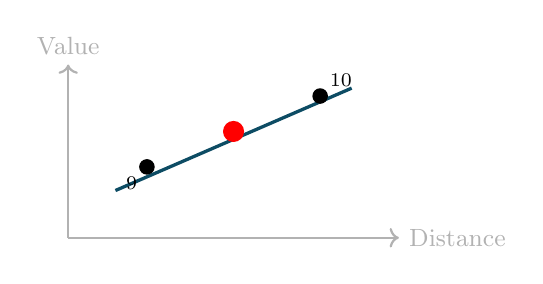
\begin{tikzpicture}[x=1.0cm,y=1.0cm]
  \draw[->, thick, gray!60] (0,0) -- (4.2,0) node[right,font=\small] {Distance};
  \draw[->, thick, gray!60] (0,0) -- (0,2.2) node[above,font=\small] {Value};
  \draw[LectureBlue, line width=1.2pt] (0.6,0.6) -- (3.6,1.9);
  \filldraw[black] (1.0,0.9) circle (2.6pt) node[below left,font=\scriptsize] {9};
  \filldraw[black] (3.2,1.8) circle (2.6pt) node[above right,font=\scriptsize] {10};
  \filldraw[red] (2.1,1.35) circle (3.6pt);
\end{tikzpicture}
\end{columns}

\vspace{1em}
\textbf{Resources \& References:}
\begin{itemize}
  \item OpenCV Implementation: \href{https://docs.opencv.org/3.4/da/d54/group__imgproc__transform.html\#ga5bb5a1fea74ea38e1a5445ca803ff121}{\color{blue}imgproc transform documentation}
  \item PyTorch Input Transforms: \href{https://pytorch.org/vision/stable/models/generated/torchvision.models.resnet50.html\#torchvision.models.resnet50}{\color{blue}Torchvision ResNet50 Specs}
  \item Further Reading: \href{https://www.mssc.mu.edu/~daniel/pubs/RoweTalkMSCS_BiCubic.pdf}{\color{blue}Bicubic Interpolation Paper (Rowe)}
\end{itemize}


\end{frame}


\begin{frame}{Interpolation Choices}
\small
\begin{tabularx}{\textwidth}{>{\bfseries}p{0.17\textwidth} >{\raggedright\arraybackslash}p{0.15\textwidth} >{\raggedright\arraybackslash}p{0.23\textwidth} X}
\toprule
Method & Support & Strengths & Use with care \\
\midrule
Nearest neighbor & 1 sample & preserves labels exactly, fastest & blocky edges in intensity images \\
Bilinear & $2 \times 2$ neighborhood & stable default for many intensity images & slight blur after repeated use \\
Bicubic & $4 \times 4$ neighborhood & smoother appearance, better edge continuity & can ring near sharp transitions \\
Spline / higher order & larger support & smooth derivatives, useful in scientific resampling & more computation and stronger assumptions \\
\bottomrule
\end{tabularx}


\end{frame}


\begin{frame}{Nearest-Neighbor Interpolation (2D)}
\begin{columns}[T,onlytextwidth]
\column{0.55\textwidth}
\small
\begin{itemize}
  \item Assigns the value of the nearest sample point to each 2D query location (constant 2D box/pixel kernel).
  \item Support: 1 nearest sample. Extremely fast.
  \item \textbf{Best for:} Segmentation masks, label maps, and discrete data (preserves exact categorical class IDs).
  \item \textbf{Avoid for:} Continuous intensity images (causes blocky/pixelated artifacts, staircasing, and is non-differentiable).
\end{itemize}

\column{0.42\textwidth}
\centering
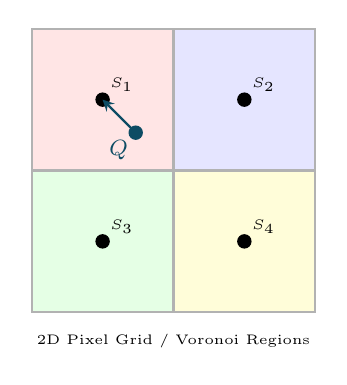
\begin{tikzpicture}[scale=1.2, font=\footnotesize]
  % Grid / Voronoi Cells (Pixel boundaries)
  \draw[gray!30, dashed] (0,0) grid (3,3);
  
  % Colored pixel regions to show "regions of influence"
  \fill[red!10] (0,1.5) rectangle (1.5,3);
  \fill[blue!10] (1.5,1.5) rectangle (3,3);
  \fill[green!10] (0,0) rectangle (1.5,1.5);
  \fill[yellow!15] (1.5,0) rectangle (3,1.5);
  
  % Cell Boundaries (Solid)
  \draw[gray!60, thick] (0,0) rectangle (3,3);
  \draw[gray!60, thick] (1.5,0) -- (1.5,3);
  \draw[gray!60, thick] (0,1.5) -- (3,1.5);
  
  % Sample Points (Pixel Centers)
  \filldraw[black] (0.75, 2.25) circle (2pt) node[above right=-1pt, font=\tiny] {$S_1$};
  \filldraw[black] (2.25, 2.25) circle (2pt) node[above right=-1pt, font=\tiny] {$S_2$};
  \filldraw[black] (0.75, 0.75) circle (2pt) node[above right=-1pt, font=\tiny] {$S_3$};
  \filldraw[black] (2.25, 0.75) circle (2pt) node[above right=-1pt, font=\tiny] {$S_4$};
  
  % Query Point
  \coordinate (Q) at (1.1, 1.9);
  \filldraw[LectureBlue] (Q) circle (2pt) node[below left=-1pt, LectureBlue] {$Q$};
  
  % Arrow to nearest neighbor
  \draw[->, LectureBlue, thick, >=stealth] (Q) -- (0.75, 2.25);
  
  % Labels
  \node[black, font=\tiny, align=center] at (1.5, -0.3) {2D Pixel Grid / Voronoi Regions};
\end{tikzpicture}
\end{columns}
\end{frame}

\begin{frame}{Bilinear Interpolation}
\begin{columns}[T,onlytextwidth]
\column{0.55\textwidth}
\small
\begin{itemize}
  \item Separable linear interpolation across a $2\times2$ neighborhood; weights depend on fractional distances $\Delta x, \Delta y \in [0, 1]$.
  
  \item \textbf{Step 1: Horizontal Interpolation}
  \begin{align*}
    f(R_1) &= (1-\Delta x)f(Q_{11}) + \Delta x f(Q_{21}) \\
    f(R_2) &= (1-\Delta x)f(Q_{12}) + \Delta x f(Q_{22})
  \end{align*}

  \item \textbf{Step 2: Vertical Interpolation}
  $$f(P) = (1-\Delta y)f(R_1) + \Delta y f(R_2)$$

  \item Continuous ($C^0$) and differentiable almost everywhere; gradients are piecewise linear.
  \item \textbf{Pros:} Computationally efficient, stable, and differentiable.
  \item \textbf{Cons:} Acts as a low-pass filter, blurring images over repeated applications.
\end{itemize}

\column{0.42\textwidth}
\centering
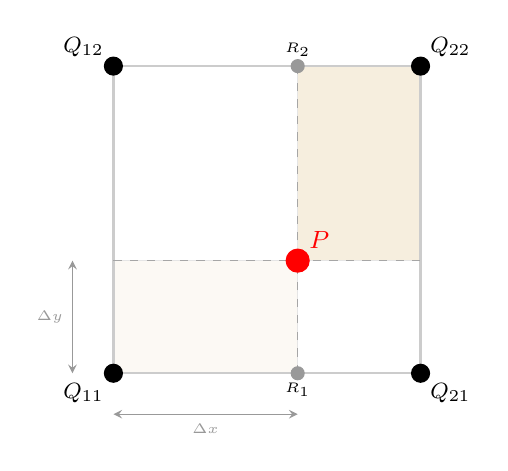
\begin{tikzpicture}[scale=1.3, font=\footnotesize]
  % Define 2x2 bounding pixel coordinates
  \coordinate (Q11) at (0,0);
  \coordinate (Q21) at (3,0);
  \coordinate (Q12) at (0,3);
  \coordinate (Q22) at (3,3);
  
  % Define Query Point P and intermediate interpolation points
  \coordinate (P) at (1.8, 1.1);
  \coordinate (R1) at (1.8, 0);
  \coordinate (R2) at (1.8, 3);

  % Draw fractional area/interpolation boxes
  \draw[gray!20, fill=LectureGold!5] (0,0) rectangle (1.8,1.1);
  \draw[gray!20, fill=LectureGold!15] (1.8,1.1) rectangle (3,3);

  % Draw the 2x2 grid cell boundaries
  \draw[gray!40, thick] (Q11) -- (Q21) -- (Q22) -- (Q12) -- cycle;
  
  % Draw 1D interpolation axis paths (Separable steps)
  \draw[dashed, gray!70] (R1) -- (R2);
  \draw[dashed, gray!70] (0,1.1) -- (3,1.1);

  % 4 Neighboring Pixel Samples
  \filldraw[black] (Q11) circle (2.5pt) node[below left] {$Q_{11}$};
  \filldraw[black] (Q21) circle (2.5pt) node[below right] {$Q_{21}$};
  \filldraw[black] (Q12) circle (2.5pt) node[above left] {$Q_{12}$};
  \filldraw[black] (Q22) circle (2.5pt) node[above right] {$Q_{22}$};

  % Intermediate Interpolation Points (Step 1)
  \filldraw[gray!80] (R1) circle (1.8pt) node[below, font=\tiny, text=black] {$R_1$};
  \filldraw[gray!80] (R2) circle (1.8pt) node[above, font=\tiny, text=black] {$R_2$};

  % Final Query Point P (Step 2)
  \filldraw[red] (P) circle (3.2pt) node[above right=1pt, red, font=\small\bfseries] {$P$};

  % Distance dimension labels
  \draw[<->, >=stealth, gray!80] (0,-0.4) -- node[below, font=\tiny] {$\Delta x$} (1.8,-0.4);
  \draw[<->, >=stealth, gray!80] (-0.4,0) -- node[left, font=\tiny] {$\Delta y$} (-0.4,1.1);
\end{tikzpicture}
\end{columns}
\end{frame}

% Slide 1: The 2D Separable Process
\begin{frame}{Bicubic Interpolation: 2D Mechanism}
\begin{columns}[T,onlytextwidth]
\column{0.55\textwidth}
\small
\begin{itemize}
    \item Extension of bilinear interpolation using a $4\times4$ neighborhood ($16$ pixels) for $C^1$ continuity.
    
    \item \textbf{Step 1: Horizontal Interpolation} \\
    Calculate 4 intermediate points $R_i$ using 1D cubic passes across rows:
    \begin{itemize}
        \scriptsize
        \item $f(R_{-1}) = \text{Cubic}(I_{-1,-1}, I_{0,-1}, I_{1,-1}, I_{2,-1}; \Delta x)$
        \item $f(R_0) \,\,= \text{Cubic}(I_{-1,0}, I_{0,0}, I_{1,0}, I_{2,0}; \Delta x)$
        \item $f(R_1) \,\,= \text{Cubic}(I_{-1,1}, I_{0,1}, I_{1,1}, I_{2,1}; \Delta x)$
        \item $f(R_2) \,\,= \text{Cubic}(I_{-1,2}, I_{0,2}, I_{1,2}, I_{2,2}; \Delta x)$
    \end{itemize}

    \item \textbf{Step 2: Vertical Interpolation} \\
    Calculate the final value at point $P$ using a vertical 1D cubic pass:
    \scriptsize
    \[ f(P) = \text{Cubic}(f(R_{-1}), f(R_0), f(R_1), f(R_2); \Delta y) \]

    \small
    \item \textbf{Result:} Smoother gradients and sharper edges compared to Bilinear, but at higher cost.
\end{itemize}

\column{0.42\textwidth}
\centering
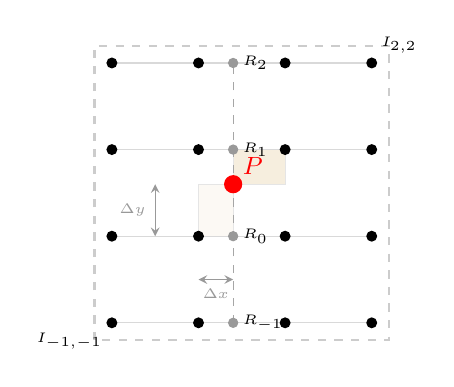
\begin{tikzpicture}[scale=1.1, font=\footnotesize]
  % Coordinates for 4x4 grid
  \foreach \x in {0,1,2,3} \foreach \y in {0,1,2,3} \coordinate (I\x\y) at (\x,\y);
  
  \coordinate (P) at (1.4, 1.6); % Target point
  
  % Interpolation boxes
  \draw[gray!20, fill=LectureGold!5] (1,1) rectangle (1.4,1.6);
  \draw[gray!20, fill=LectureGold!15] (1.4,1.6) rectangle (2,2);

  \draw[gray!40, thick, dashed] (-0.2,-0.2) rectangle (3.2,3.2);
  
  % Grid lines
  \foreach \y in {0,1,2,3} \draw[gray!30, thin] (0,\y) -- (3,\y);
  \draw[dashed, gray!70] (1.4, 0) -- (1.4, 3); % Vertical Step 2 line

  % Neighbor samples
  \foreach \x in {0,1,2,3} \foreach \y in {0,1,2,3} \fill[black] (\x,\y) circle (1.8pt);
  
  % Labels
  \node[below left, font=\tiny] at (0,0) {$I_{-1,-1}$};
  \node[above right, font=\tiny] at (3,3) {$I_{2,2}$};

  % Intermediate R Points
  \foreach \y [count=\i from -1] in {0,1,2,3} {
    \filldraw[gray!80] (1.4,\y) circle (1.5pt) node[right, font=\tiny, text=black] {$R_{\i}$};
  }

  % Final Point P
  \filldraw[red] (P) circle (2.8pt) node[above right, red, font=\small\bfseries] {$P$};

  % Distances
  \draw[<->, >=stealth, gray!80] (1, 0.5) -- node[below, font=\tiny] {$\Delta x$} (1.4, 0.5);
  \draw[<->, >=stealth, gray!80] (0.5, 1) -- node[left, font=\tiny] {$\Delta y$} (0.5, 1.6);
\end{tikzpicture}
\end{columns}
\end{frame}

% Slide 2: The Cubic Kernel Math
\begin{frame}{Bicubic Interpolation: The Cubic Function}
\begin{columns}[T,onlytextwidth]
\column{0.55\textwidth}
\small
\begin{itemize}
    \item The $\text{Cubic}(p_{-1}, p_0, p_1, p_2; x)$ function fits a 3rd-degree polynomial through 4 points.
    \item Typically uses the \textbf{Catmull-Rom} spline to ensure the curve passes through $p_0$ and $p_1$ while maintaining slope continuity.
    
    \item \textbf{Polynomial Form:}
    \[ f(x) = a_3x^3 + a_2x^2 + a_1x + a_0 \]
    
    \item \textbf{Key Trait:} Unlike linear weight (straight lines), cubic weights can be negative, leading to "overshoot" which increases perceived sharpness.
\end{itemize}

\column{0.42\textwidth}
\centering
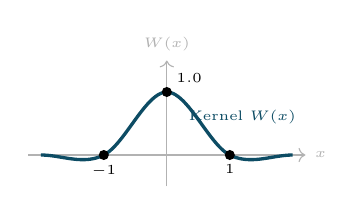
\begin{tikzpicture}[scale=0.8]
    % Draw the Cubic Kernel Shape (Catmull-Rom)
    \draw[->, gray!60] (-2.2,0) -- (2.2,0) node[right, font=\tiny] {$x$};
    \draw[->, gray!60] (0,-0.5) -- (0,1.5) node[above, font=\tiny] {$W(x)$};
    
    % The kernel curve
    \draw[LectureBlue, very thick, samples=100, domain=-2:2] plot (\x, {
        abs(\x) <= 1 ? (1.5*abs(\x)^3 - 2.5*abs(\x)^2 + 1) : 
        (abs(\x) <= 2 ? (-0.5*abs(\x)^3 + 2.5*abs(\x)^2 - 4*abs(\x) + 2) : 0)
    });
    
    % Node labels
    \filldraw[black] (0,1) circle (2pt) node[above right, font=\tiny] {$1.0$};
    \filldraw[black] (1,0) circle (2pt) node[below, font=\tiny] {$1$};
    \filldraw[black] (-1,0) circle (2pt) node[below, font=\tiny] {$-1$};
    \node[LectureBlue, font=\tiny] at (1.2,0.6) {Kernel $W(x)$};
\end{tikzpicture}
\vfill
\scriptsize\textcolor{gray}{Note: Matrix coefficients map pixels to the range $[0, 1]$ relative to the central interval.}
\end{columns}
\end{frame}

\begin{frame}{Cubic Spline: Derivative-Based Formulation}
\begin{columns}[T,onlytextwidth]
\column{0.55\textwidth}
\small
\begin{itemize}
    \item Instead of using specialized basis functions, we fit a standard third-degree polynomial between pixels $p_0$ and $p_1$:
    \[ f(x) = ax^3 + bx^2 + cx + d \]
    where $x \in$ is the fractional distance.

    \item \textbf{1. Setting up the Constraints:} \\
    To find the 4 unknown coefficients ($a, b, c, d$), we enforce 4 conditions based on pixel values and their slopes ($m_0, m_1$):
    \begin{itemize}
        \scriptsize
        \item \textbf{Value at $x=0$:} $f(0) = d = p_0$
        \item \textbf{Value at $x=1$:} $f(1) = a + b + c + d = p_1$
        \item \textbf{Slope at $x=0$:} $f'(0) = c = m_0$
        \item \textbf{Slope at $x=1$:} $f'(1) = 3a + 2b + c = m_1$
    \end{itemize}

    \small
    \item \textbf{2. Solving for the Coefficients:} \\
    Solving this system of linear equations yields:
    \scriptsize
    \begin{align*}
        a &= 2p_0 - 2p_1 + m_0 + m_1 \\
        b &= -3p_0 + 3p_1 - 2m_0 - m_1 \\
        c &= m_0 \\
        d &= p_0
    \end{align*}

\end{itemize}

\column{0.42\textwidth}
\centering
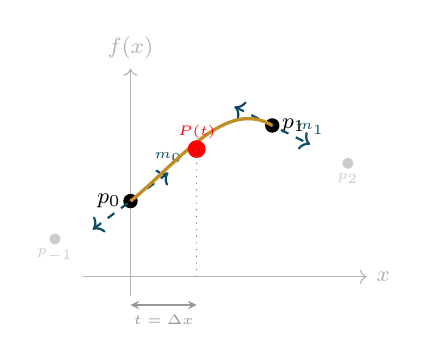
\begin{tikzpicture}[scale=1.2, font=\footnotesize]
    % Axes
    \draw[->, gray!60] (-0.5,0) -- (2.5,0) node[right] {$x$};
    \draw[->, gray!60] (0,-0.2) -- (0,2.2) node[above] {$f(x)$};

    % Control Points
    \coordinate (Pm1) at (-0.8, 0.4);
    \coordinate (P0)  at (0, 0.8);
    \coordinate (P1)  at (1.5, 1.6);
    \coordinate (P2)  at (2.3, 1.2);

    % Draw support points (ghost points)
    \filldraw[gray!40] (Pm1) circle (1.5pt) node[below, font=\tiny] {$p_{-1}$};
    \filldraw[gray!40] (P2)  circle (1.5pt) node[below, font=\tiny] {$p_{2}$};

    % Main segment points
    \filldraw[black] (P0) circle (2pt) node[left] {$p_0$};
    \filldraw[black] (P1) circle (2pt) node[right] {$p_1$};

    % Tangent lines (Derivatives)
    \draw[dashed, LectureBlue, thick, <->] (-0.4, 0.5) -- (0.4, 1.1) node[above, font=\tiny] {$m_0$};
    \draw[dashed, LectureBlue, thick, <->] (1.1, 1.8) -- (1.9, 1.4) node[above, font=\tiny] {$m_1$};

    % The Spline Curve
    \draw[LectureGold, very thick] (P0) .. controls (0.5, 1.2) and (1.0, 1.9) .. (P1);

    % Query Point P(t)
    \coordinate (Pt) at (0.7, 1.35);
    \filldraw[red] (Pt) circle (2.5pt) node[above, font=\tiny\bfseries] {$P(t)$};
    
    % Distance Label
    \draw[<->, >=stealth, gray!80] (0, -0.3) -- node[below, font=\tiny] {$t = \Delta x$} (0.7, -0.3);
    \draw[dotted, gray] (0.7,0) -- (Pt);
\end{tikzpicture}

\vfill
\scriptsize\textcolor{gray}{Visual: Derivatives $m_0, m_1$ control the shape/curvature of the segment between $p_0$ and $p_1$.}
\vfill
\vspace{1em}

\textbf{Slopes ($m_i$):} Usually estimated from neighboring pixels via central differences: $m_0 = \frac{p_1 - p_{-1}}{2}$.
\vspace{1em}

\textbf{Benefit:} This ensures \textbf{$C^1$ continuity} (the slope is the same on both sides of a pixel), preventing visible "seams" in upscaled images.
\end{columns}
\end{frame}

\begin{frame}{Interpolation as a Kernel Model}
\begin{columns}[T,onlytextwidth]
\column{0.58\textwidth}
\[
I(x,y) = \sum_{m,n} I[m,n] \, \phi(x-m)\,\phi(y-n)
\]
\vspace{-0.6em}
\begin{itemize}
\item Interpolation is a choice of basis or kernel $\phi$ on the discrete grid.
\item Nearest neighbor uses a box-like basis.
\item Bilinear uses a triangular basis.
\item Cubic methods use smoother kernels with wider support.
\end{itemize}



\column{0.36\textwidth}
\centering
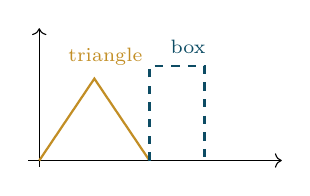
\begin{tikzpicture}[x=0.7cm,y=0.8cm]
\draw[->] (-0.2,0) -- (4.4,0);
\draw[->] (0,-0.1) -- (0,2.1);
\draw[LectureGold,thick] (0,0) -- (1,1.3) -- (2,0);
\draw[LectureBlue,thick,dashed] (2,0) -- (2,1.5) -- (3,1.5) -- (3,0);
\node[font=\scriptsize,LectureGold] at (1.2,1.65) {triangle};
\node[font=\scriptsize,LectureBlue] at (2.7,1.8) {box};
\end{tikzpicture}

\href{https://www.youtube.com/watch?v=Xj129kA3Ci0}{\color{blue}Animation}

\end{columns}

\end{frame}

\begin{frame}{Interpolation Has a Spectral Interpretation}
\begin{columns}[T,onlytextwidth]
\column{0.53\textwidth}
\begin{itemize}
\item Every interpolation kernel has a transfer function in frequency.
\item Nearest neighbor preserves edges aggressively but leaks high-frequency artifacts.
\item Bilinear is smoother but attenuates high frequencies more strongly.
\item Higher-order kernels can better preserve smooth structure but may introduce ringing.
\end{itemize}


\column{0.41\textwidth}
\centering
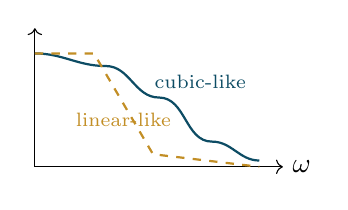
\begin{tikzpicture}[x=0.75cm,y=0.8cm]
\draw[->] (0,0) -- (4.2,0) node[right] {$\omega$};
\draw[->] (0,0) -- (0,2.2);
\draw[LectureBlue,thick] (0,1.8) to[out=0,in=180] (1.2,1.6) to[out=0,in=180] (2.1,1.1) to[out=0,in=180] (3.0,0.4) to[out=0,in=180] (3.8,0.1);
\draw[LectureGold,thick,dashed] (0,1.8) -- (1.0,1.8) -- (2.0,0.2) -- (3.8,0.0);
\node[font=\scriptsize,LectureBlue] at (2.8,1.35) {cubic-like};
\node[font=\scriptsize,LectureGold] at (1.5,0.75) {linear-like};
\end{tikzpicture}
\end{columns}
\end{frame}


\begin{frame}{Labels Are Not Intensities}
\begin{columns}[T,onlytextwidth]
\column{0.50\textwidth}
\begin{itemize}
\item A grayscale image encodes ordered numeric intensity.
\item A segmentation mask encodes categorical identity.
\item Linear interpolation between labels 1 and 3 producing 2 is usually meaningless.
\end{itemize}

\column{0.44\textwidth}
\small
\begin{tabularx}{\linewidth}{>{\bfseries}p{0.35\linewidth} X}
\toprule
Data type & Typical interpolation \\
\midrule
Intensity image & linear or cubic \\
Label map & nearest neighbor \\
\bottomrule
\end{tabularx}
\end{columns}
\end{frame}



\begin{frame}{Deep Learning Still Depends on Classical Image Manipulation}
\begin{columns}[T,onlytextwidth]
\column{0.32\textwidth}
\begin{block}{Preprocessing}
\begin{itemize}
\item resize or crop to fixed input shapes
\item normalize intensity after choosing a display or physical range
\item standardize spacing across scanners or sites
\end{itemize}
\end{block}

\column{0.32\textwidth}
\begin{block}{Augmentation}
\begin{itemize}
\item flips, rotations, zoom, and elastic warps
\item label geometry must follow the image exactly
\end{itemize}
\end{block}

\column{0.32\textwidth}
\begin{block}{Learnable geometry}
\begin{itemize}
\item Spatial Transformer Networks predict a warp and then resample differentiably
\item the grid sampler is classical interpolation inside a neural network
\item modern models still inherit the same resampling trade-offs
\end{itemize}
\end{block}
\end{columns}
\end{frame}

\begin{frame}{Differentiable Resampling Inside Neural Networks}
\small
Spatial Transformer Networks use a learned transform and a differentiable sampler. For bilinear sampling,

\[
V_i^c = \sum_n \sum_m U_{nm}^c \max(0,1-|x_i^s-m|)\max(0,1-|y_i^s-n|)
\]

\begin{itemize}
\item $U$: input feature map, $V$: output feature map
\item $(x_i^s, y_i^s)$: sampled source coordinate predicted by the network
\item The sampler is modern deep learning built on classical interpolation
\end{itemize}

\begin{alertblock}{Important perspective}
Neural networks can learn where to sample, but they still inherit the mathematical biases of the interpolation kernel.
\end{alertblock}
\end{frame}

\begin{frame}{Spatial Transformer Networks (STN) [cite: 150]}
    \textbf{Global Learnable Geometry} [cite: 151]\\
    Jaderberg et al. (2015) introduced the STN as a modular component that allows a network to actively transform data spatially. [cite: 152]
    
    \vspace{0.5em}
    \begin{itemize}
        \item \textbf{Localisation Net:} Regresses transformation parameters $\theta$ (e.g., affine, TPS). [cite: 153]
        \item \textbf{Grid Generator:} Produces a sampling grid based on $\theta$. [cite: 154]
        \item \textbf{Sampler:} Interpolates input at the generated grid points. [cite: 155]
    \end{itemize}
\end{frame}

\begin{frame}{The Differentiable Sampler [cite: 169]}
    For a network to learn geometry via backpropagation, the sampling must be differentiable. [cite: 170]\\
    \vspace{0.5em}
    Bilinear sampling for a target pixel $V_i$ at source location $(x_i,y_i)$[cite: 171]:
    $$V_{i}^{c}=\sum_{n}\sum_{m}U_{nm}^{c}\max(0,1-|x_{i}^{s}-m|)\max(0,1-|y_{i}^{s}-n|)$$ [cite: 172]
    
    \textbf{Forward Pass} [cite: 173]\\
    Classic bilinear interpolation but the coordinates are outputs of a previous layer, not a fixed scaling factor. [cite: 174]\\
    \vspace{0.5em}

    \textbf{Backward Pass} [cite: 175]\\
    Partial derivatives $\frac{\partial V}{\partial x}$ and $\frac{\partial V}{\partial y}$ allow the network to "push" sampling points toward features that minimize loss. [cite: 176]
\end{frame}

\begin{frame}{Deformable Convolutions (DCN) [cite: 177]}
    \textbf{Local vs. Global Geometry} [cite: 178]\\
    While STN applies a global warp, Deformable CNNs (Dai et al., 2017) learn local offsets for every convolution kernel position. [cite: 179]
    
    \vspace{0.5em}
    \begin{itemize}
        \item The receptive field adapts to object shape. [cite: 180]
        \item Offsets $\Delta p_n$ are learned via an auxiliary convolution branch. [cite: 181]
        \item Crucial for non-rigid objects and varying perspectives. [cite: 182]
    \end{itemize}
\end{frame}

\begin{frame}{DCN: Mathematical Offset Logic [cite: 184]}
    In a standard convolution, the output $y(p_0)$ is a weighted sum over a fixed grid $R$. [cite: 185]\\
    In DCN, we add a fractional offset $\Delta p_n$[cite: 186]:
    $$y(p_{0})=\sum_{p_{n}\in R}w(p_{n})\cdot x(p_{0}+p_{n}+\Delta p_{n})$$ [cite: 187]
    \vspace{1em}

    \begin{table}[]
    \centering
    \resizebox{\textwidth}{!}{%
    \begin{tabular}{|l|l|l|}
    \hline
    \textbf{Component} & \textbf{Standard Convolution} & \textbf{Deformable Convolution} \\ \hline
    Sampling Grid & Fixed (e.g., $3 \times 3$) & Arbitrary (Learnable offsets) \\ \hline
    Receptive Field & Constant Shape & Data-adaptive Shape \\ \hline
    Interpolation & Not Required (on-grid) & Required (Bilinear at offsets) \\ \hline
    \end{tabular}%
    }
    \end{table} [cite: 188]
\end{frame}

\begin{frame}{Implicit Neural Representations (INR) [cite: 189]}
    \textbf{Continuous Digital Signal} [cite: 190]\\
    Instead of storing pixels, we learn a function $f_{\theta}: \mathbb{R}^2 \rightarrow \mathbb{R}^3$ that maps coordinates to values. [cite: 191, 192]
    
    \vspace{0.5em}
    \begin{itemize}
        \item Infinite resolution potential. [cite: 193]
        \item Differentiable with respect to space. [cite: 194]
        \item No discrete kernel-the MLP is the interpolator. [cite: 195]
    \end{itemize}
\end{frame}

\begin{frame}{Regularizing Geometric Learning [cite: 200]}
    Unconstrained learning of transformations leads to self-intersecting grids and unrealistic artifacts. We enforce smoothness via regularization: [cite: 201]
    \vspace{1em}

    \textbf{Total Variation (TV)} [cite: 202]\\
    Prevents jerky, non-smooth displacement fields. Essential for visual consistency. [cite: 206]
    $$L_{smooth}=\int||\nabla\phi(x)||^{2}dx$$ [cite: 203]

    \textbf{Bending Energy} [cite: 204]\\
    Derived from Thin-Plate Splines. Penalizes second-order curvature to ensure diffeomorphic maps. [cite: 207]
    $$L_{bend}=\int||\nabla^{2}\phi(x)||^{2}dx$$ [cite: 205]
\end{frame}

\begin{frame}{Medical Image Registration [cite: 208]}
    \textbf{Learnable Elastic Warps} [cite: 209]\\
    In medical imaging, we often need to align a Source image to a Target (e.g., pre-op vs. post-op). [cite: 210]
    
    \vspace{0.5em}
    \begin{itemize}
        \item Classical methods (Demons, B-Splines) are slow optimization loops. [cite: 211]
        \item Deep models (VoxelMorph) learn a global function that predicts the displacement field in milliseconds, treating registration as a feed-forward inference task. [cite: 212]
    \end{itemize}
    \vspace{1em}
    \textit{PhD Note: The grid sampler here acts as a physical constraint-the image cannot "break" if the warp is diffeomorphic.} [cite: 213]
\end{frame}


\begin{frame}{Suggested Reading}
\small
\begin{itemize}
\item R. C. Gonzalez and R. E. Woods, \emph{Digital Image Processing}, 3rd ed.
\item R. Szeliski, \emph{Computer Vision: Algorithms and Applications}, 2nd ed.
\item M. Jaderberg et al., \emph{Spatial Transformer Networks}, NeurIPS 2015.
\item J. A. Fessler, \emph{Fundamentals of Image Reconstruction}, for a stronger operator viewpoint.
\end{itemize}

\vspace{1em}
\begin{block}{Final discussion prompt}
If a model input must be resized from $512 \times 512$ to $224 \times 224$, which information is lost, which information can be partially approximated by a model, and which scientific claims become harder to justify afterward?
\end{block}
\end{frame}

\end{document}
